% !TeX program = xelatex
\documentclass[12pt,a4paper,openany]{book}
\usepackage{fontspec}
\usepackage{polyglossia}
\setdefaultlanguage{german}
\setotherlanguage{arabic}
\newfontfamily\arabicfont[Script=Arabic,Scale=1.1]{Amiri}
\usepackage{geometry}
\geometry{a4paper, margin=2.2cm}
\usepackage{yalla}
\usepackage[colorlinks=true, linkcolor=yallateal, urlcolor=yallared, citecolor=yallateal]{hyperref}
\usepackage{titlesec}
\titleformat{\chapter}[display]{\normalfont\huge\bfseries\color{yallanight}}{Teil \thechapter}{10pt}{\Huge}
\titlespacing*{\chapter}{0pt}{0pt}{30pt}
\usepackage{fancyhdr}
\setlength{\headheight}{15pt}
\pagestyle{fancy}
\fancyhf{}
\fancyhead[LE,RO]{\thepage}
\fancyhead[RE]{\textit{Yalla, Julia!}}
\fancyhead[LO]{\leftmark}
\renewcommand{\headrulewidth}{0.4pt}
\title{\Huge\bfseries\color{yallanight}Yalla, Julia!\\[6pt]\Large\color{yallared}Arabisch für Ägypten\\[4pt]\large\color{yallanight}Band 1 -- Die Buchstaben \& das Überleben}
\author{ein Projekt von Mohamed, für Julia \faHeart}
\date{A1 \ -- \ Version 1.1}
\begin{document}
\frontmatter
\begin{titlepage}
\centering
\vspace*{1cm}
\yallarule
\vspace{1.5cm}
{\Huge\bfseries\color{yallanight} Yalla, Julia! \faSmileWink}\\[10pt]
{\Large\color{yallared} Arabisch für Ägypten}\\[6pt]
{\large\color{yallanight} Band 1 -- Die Buchstaben \& das Überleben}\\[4pt]
{\normalsize\itshape Niveau A1 -- Version 1.1}
\vspace{2cm}
\textarabic{\bigletterfont\fontsize{40}{40}\selectfont مرحباً يا جوليا}
\vspace{1.5cm}
{\normalsize für Julia -- mit viel Liebe (und ein bisschen kontrolliertem Chaos)}
\vfill
\yallarule
\end{titlepage}
\tableofcontents

\chapter*{Teil 0 -- Wie dieses Buch funktioniert}
\addcontentsline{toc}{chapter}{Teil 0 -- Wie dieses Buch funktioniert}
\markboth{Wie dieses Buch funktioniert}{}

Liebe Julia,

das hier ist kein Lehrbuch, das dich langweilen will. Es ist eine Einladung:
an Straßenschilder, Taxifahrer, Kaffeehausbesitzer und mindestens eine sehr
selbstbewusste Straßenkatze namens Bisso. Los geht's -- ganz von vorne, ganz
in Ruhe.

\section*{Was du hier lernst: ganz normales, gesprochenes Arabisch}

Arabisch hat zwei Ebenen: eine Schriftsprache für Nachrichten und Bücher
(Fus'Ha), und die Sprache, die 90 Millionen Menschen in Kairo tatsächlich
\emph{sprechen} (Masri, Ägyptisch-Arabisch). \textbf{Dieses Buch
konzentriert sich fast komplett auf Masri} -- das normale, entspannte
Alltagsarabisch, das du beim Taxifahren, im Café und beim Feilschen
brauchst. Nur an wenigen Stellen zeigen wir dir kurz den Fus'Ha-Unterschied,
falls du ihn mal auf einem Schild siehst.

\begin{tippbox}
Du musst dir jetzt noch \emph{gar keine} Sorgen um ,,zwei Sprachen`` machen.
Für den Anfang gilt: lern die Wörter in diesem Buch so, wie sie dastehen --
das ist genau das Arabisch, das echte Menschen in Ägypten mit dir sprechen
werden.
\end{tippbox}

\section*{Die Julia-Umschrift}

Arabisch hat Laute, die es im Deutschen nicht gibt -- aber du hast einen
Heimvorteil: Deutsch besitzt bereits zwei Laute, an denen Englischsprachige verzweifeln.

\begin{center}
\renewcommand{\arraystretch}{1.4}
\begin{tabular}{cll}
\textbf{Zeichen} & \textbf{Beispiel} & \textbf{Eselsbrücke} \\
\hline
ch & \textit{chal\'as} & wie \textbf{ch} in ,,Ba\textbf{ch}`` \\
sch & \textit{sch\'ukran} & wie \textbf{sch} in ,,\textbf{Sch}ule`` \\
g & \textit{gam\'il} & wie \textbf{g} in ,,\textbf{g}eben`` -- ägyptisch, nie ,,dsch``! \\
' & \textit{'ahwa} & ein kleiner Stopp, wie in ,,Spiegel-\textbf{ei}`` \\
3 & \textit{3\'ayez} & ein Laut tief aus dem Hals \\
H & \textit{aHmed} & ein heißes, geflüstertes H \\
\end{tabular}
\end{center}

Betonte Silben tragen einen Akzent (\textit{chal\'as}). Mehr brauchst du
nicht, um loszulegen.

\section*{Die Symbole in diesem Buch}

\begin{center}
\renewcommand{\arraystretch}{1.5}
\begin{tabular}{cl}
\textcolor{yallateal}{\faVolumeUp} & Tippen -> Google Translate öffnet sich -> Lautsprecher-Symbol tippen -> hören \\
\faHeart & Mohameds eigene Stimme (folgt in einer späteren Version) \\
\faLightbulb & Insider-Tipp für Ägypten \\
\faSmileWink & Lach-Pause \\
\faTaxi & Am Mahmoud, der Taxifahrer, hat etwas zu sagen \\
\faPaw & Bisso, die Straßenkatze, hat eine Meinung \\
\faFlagCheckered & Checkpoint -- kurz prüfen, ob's sitzt \\
\end{tabular}
\end{center}

\begin{tippbox}
Das \textcolor{yallateal}{\faVolumeUp}-Symbol öffnet Google Translate mit
dem Wort schon eingetragen -- Standardaussprache, sehr nützlich, aber nicht
immer der ägyptische Klang. Für die Wörter mit \faHeart\ gibt es später
eine Aufnahme von genau der Person, mit der du sie eigentlich sprechen
willst. Zum Antippen brauchst du eine Internetverbindung und einen
PDF-Betrachter, der Links öffnet (z.B. am Handy oder im Browser).
\end{tippbox}

\section*{Die Besetzung}

\begin{ammahmoudbox}
\textbf{Am Mahmoud} fährt seit 30 Jahren Taxi in Kairo, kennt jeden Umweg
und jeden Trick, und ist der Meinung, dass jeder Preis Verhandlungssache
ist. Sein Porträt folgt in einer späteren Version.
\end{ammahmoudbox}

\begin{bissobox}
\textbf{Bisso} ist eine Straßenkatze mit einer eingekerbten Ohrspitze und
starken Meinungen zu Essensresten.
\end{bissobox}

\begin{center}
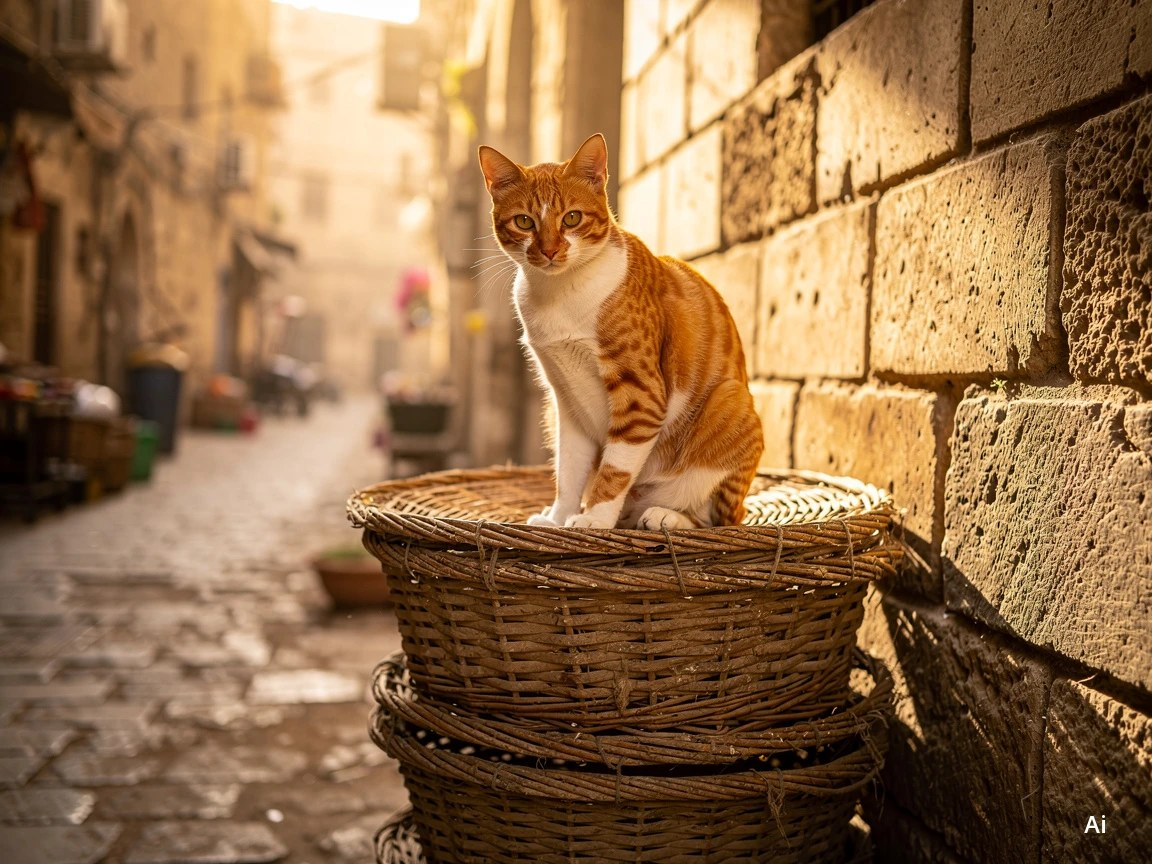
\includegraphics[width=0.5\textwidth]{images/bisso.jpg}\\
{\small\itshape Bisso, wie sie wirklich aussieht (ja, wirklich).}
\end{center}

Bereit? \textarabic{يلا بينا!} (\textit{yalla beena} -- ,,los geht's, wir beide!``)

\mainmatter

\chapter{Buchstaben-Werkstatt I -- Die Verbinder}

Fünf Buchstaben, ein Skelett: \arbig{ب} \arbig{ت} \arbig{ث} \arbig{ن} \arbig{ي}
sehen sich in der Wortmitte alle sehr ähnlich -- ein kleiner ,,Zahn``. Was
sie unterscheidet, sind nur die Punkte.

\begin{lachbox}
Stell dir eine Familie von fünf Geschwistern vor, die alle das gleiche
T-Shirt tragen -- man erkennt sie nur an den Punkten, die sie sich ins
Gesicht gemalt haben. Das ist \arbig{ب ت ث ن ي}.
\end{lachbox}

\section*{ب -- baa}
Ein Punkt darunter.
\begin{center}
\begin{tabular}{ll}
\textbf{Allein:} & \arbig{ب} \\
\textbf{Anfang:} & \textarabic{\Large بيت} \quad bayt (Haus) \\
\textbf{Mitte:} & \textarabic{\Large كبير} \quad kab\'ir (groß) \\
\textbf{Ende:} & \textarabic{\Large طبيب} \quad Tab\'ib (Arzt) \\
\end{tabular}
\end{center}
\tracerow{ب}

\section*{ت -- taa}
Zwei Punkte darüber.
\begin{center}
\begin{tabular}{ll}
\textbf{Allein:} & \arbig{ت} \\
\textbf{Anfang:} & \textarabic{\Large تفاح} \quad tuff\'aH (Apfel) \\
\textbf{Mitte:} & \textarabic{\Large كتاب} \quad kit\'ab (Buch) \\
\textbf{Ende:} & \textarabic{\Large بنت} \quad bint (Mädchen) \\
\end{tabular}
\end{center}
\tracerow{ت}

\section*{ث -- thaa}
Drei Punkte darüber. Ein seltener Gast im Alltag -- diese zwei Wörter
reichen für den Anfang völlig.
\begin{center}
\begin{tabular}{ll}
\textbf{Allein:} & \arbig{ث} \\
\textbf{Anfang:} & \textarabic{\Large ثلاجة} \quad tal\'aaga (Kühlschrank) \\
\textbf{Mitte:} & \textarabic{\Large كتير} \quad kit\'ir (viel/sehr -- kennst du schon!) \\
\end{tabular}
\end{center}
\tracerow{ث}

\section*{ن -- nuun}
Ein Punkt darüber, tiefere Schale.
\begin{center}
\begin{tabular}{ll}
\textbf{Allein:} & \arbig{ن} \\
\textbf{Anfang:} & \textarabic{\Large نور} \quad nuur (Licht) \\
\textbf{Mitte:} & \textarabic{\Large كنافة} \quad kunaafa (das Dessert!) \\
\textbf{Ende:} & \textarabic{\Large لبن} \quad laban (Milch) \\
\end{tabular}
\end{center}
\tracerow{ن}

\begin{tippbox}
كنافة (kunaafa) ist ein warmes, sirupsüßes Gebäck mit Käse oder Sahne --
DER Grund, im Ramadan hungrig zu bleiben. Merk dir das Wort.
\end{tippbox}

\section*{ي -- yaa}
Zwei Punkte darunter, Schwanz am Ende.
\begin{center}
\begin{tabular}{ll}
\textbf{Allein:} & \arbig{ي} \\
\textbf{Anfang:} & \textarabic{\Large ياسمين} \quad yasm\'in (Jasmin) \\
\textbf{Mitte:} & \textarabic{\Large بيت} \quad bayt (Haus, y in der Mitte) \\
\textbf{Ende:} & \textarabic{\Large كرسي} \quad kursi (Stuhl) \\
\end{tabular}
\end{center}
\tracerow{ي}

\begin{checkpointbox}
Kannst du \arbig{ب}, \arbig{ت}, \arbig{ث}, \arbig{ن} und \arbig{ي} in einem
Wort wiedererkennen, nur an den Punkten? Wenn ja: weiter zu Teil 2!
\end{checkpointbox}


\chapter{Buchstaben-Werkstatt II -- Die Sturköpfe}

Diese sechs Buchstaben sind Einzelgänger: \arbig{ا} \arbig{و} \arbig{ر}
\arbig{ز} \arbig{د} \arbig{ذ} geben zwar gerne eine Hand nach hinten,
weigern sich aber, nach vorne eine zweite Hand auszustrecken.

\begin{lachbox}
Das sind die Sturköpfe der Familie: sie hören zu (verbinden sich mit dem,
was davor kommt), aber sie antworten nie (verbinden sich nie mit dem, was
danach kommt). Ziemlich deutsches Verhalten, eigentlich.
\end{lachbox}

\section*{ا -- alif}
\begin{center}
\begin{tabular}{ll}
\textbf{Allein / Anfang:} & \arbig{ا} \\
\textbf{Nach einem Buchstaben:} & \textarabic{\Large بابا} \quad baaba (Papa) \\
\end{tabular}
\end{center}
\tracerow{ا}

\section*{و -- waaw}
\begin{center}
\begin{tabular}{ll}
\textbf{Allein / Anfang:} & \arbig{و} \quad \textarabic{\Large ورد} \quad ward (Rose) \\
\textbf{Nach einem Buchstaben:} & \textarabic{\Large أبو} \quad abu (Vater von...) \\
\end{tabular}
\end{center}
\tracerow{و}

\section*{ر -- raa}
\begin{center}
\begin{tabular}{ll}
\textbf{Allein / Anfang:} & \arbig{ر} \quad \textarabic{\Large ورد} \quad ward (Rose, r in der Mitte) \\
\textbf{Nach einem Buchstaben:} & \textarabic{\Large قمر} \quad qamar (Mond) \\
\end{tabular}
\end{center}
\tracerow{ر}

\section*{ز -- zaay}
\begin{center}
\begin{tabular}{ll}
\textbf{Allein / Anfang:} & \arbig{ز} \quad \textarabic{\Large زهرة} \quad zahra (Blume) \\
\textbf{Nach einem Buchstaben:} & \textarabic{\Large موز} \quad mooz (Banane) \\
\end{tabular}
\end{center}
\tracerow{ز}

\begin{tippbox}
موز (mooz) -- Banane. Ja, wirklich, es klingt fast wie im Deutschen mit
Akzent. Ägyptische Bananen sind kleiner und süßer -- probier sie.
\end{tippbox}

\section*{د -- daal}
\begin{center}
\begin{tabular}{ll}
\textbf{Allein / Anfang:} & \arbig{د} \quad \textarabic{\Large دار} \quad daar (Haus/Anwesen) \\
\textbf{Nach einem Buchstaben:} & \textarabic{\Large ولد} \quad walad (Junge) \\
\end{tabular}
\end{center}
\tracerow{د}

\section*{ذ -- dhaal}
Selten im Alltag -- im Masri wird daraus meist ein ,,d`` oder ,,z``.
\begin{center}
\begin{tabular}{ll}
\textbf{Allein / Anfang:} & \arbig{ذ} \\
\textbf{Nach einem Buchstaben:} & \textarabic{\Large هذا} \quad haadha (dieses hier; Masri oft: \emph{da}) \\
\end{tabular}
\end{center}
\tracerow{ذ}

\begin{checkpointbox}
Merksatz: \arbig{ا و ر ز د ذ} geben nie eine zweite Hand. Nach ihnen fängt
jeder Buchstabe wieder ganz von vorne an -- das ist Absicht, kein
Druckfehler!
\end{checkpointbox}


\chapter{Die kleinen Helfer -- Vokale}

Arabisch schreibt normalerweise nur die Konsonanten und langen Vokale.
Die kurzen Vokale (a, i, u) werden meist \emph{nicht} geschrieben -- du musst
sie lernen wie Melodien. In Lehrbüchern (und hier) setzen wir sie aber als
kleine Hilfszeichen über oder unter den Buchstaben.

\begin{center}
\renewcommand{\arraystretch}{2}
\begin{tabular}{cccl}
\textbf{Name} & \textbf{Lage} & \textbf{Beispiel} & \textbf{Klingt wie} \\
\hline
Fatha & Strich oben & \textarabic{\Large بَ} (ba) & kurzes a \\
Kasra & Strich unten & \textarabic{\Large بِ} (bi) & kurzes i \\
Damma & Komma oben & \textarabic{\Large بُ} (bu) & kurzes u \\
Sukun & Kringel oben & \textarabic{\Large بْ} (b) & gar kein Vokal \\
Shadda & kleines w oben & \textarabic{\Large بّ} (bb) & doppelter Konsonant \\
\end{tabular}
\end{center}

\begin{lachbox}
Fatha sieht aus wie ein kleiner, gefallener Schnurrbart über dem
Buchstaben. Kasra ist derselbe Schnurrbart, nur er ist heruntergefallen
und liegt jetzt unten. Damma ist ein winziges Ohr, das nach oben lauscht.
\end{lachbox}

\section*{Die drei langen Vokale}

Lange Vokale werden dagegen tatsächlich als eigene Buchstaben geschrieben:
\arbig{ا} für langes \emph{aa}, \arbig{و} für langes \emph{uu}, \arbig{ي}
für langes \emph{ii}.

\begin{center}
\begin{tabular}{ll}
langes \textit{aa}: & \textarabic{\Large كتاب} \quad kit\'ab (Buch) \\
langes \textit{uu}: & \textarabic{\Large دور} \quad duur (Rollen/Runden) \\
langes \textit{ii}: & \textarabic{\Large كبير} \quad kab\'ir (groß) \\
\end{tabular}
\end{center}

\begin{tippbox}
Ein Wort, das du garantiert brauchen wirst: \textarabic{\Large حبيبي} --
\textit{Hab\'ibi} -- ,,mein Schatz/Liebling``. Langes \textit{ii} mitten
im Wort. Wenn Mohamed dich so nennt, weißt du jetzt auch, warum es sich
so lang anhört.
\end{tippbox}

\section*{Kurzer Vergleich}

\begin{center}
\begin{tabular}{lll}
\textarabic{\Large كتاب} kit\'ab & (ein) Buch & mit langem a \\
\textarabic{\Large كُتُب} kutub & Bücher (Plural!) & mit kurzem u, u \\
\end{tabular}
\end{center}

\begin{checkpointbox}
Du musst die Vokalzeichen nicht auswendig zeichnen können -- du musst sie
nur \emph{erkennen}. Im echten Alltag (Straßenschilder, WhatsApp)
verschwinden sie fast komplett -- Muttersprachler lesen Arabisch meistens
ohne sie, so wie du ,,Str.`` automatisch als ,,Straße`` liest.
\end{checkpointbox}


\chapter{Überleben I -- Die Begrüßungs-Choreografie}

In Ägypten ist eine Begrüßung kein einzelnes Wort -- es ist ein kleines
Ritual mit festen Schritten, wie ein Tanz. Wenn du den ersten Schritt
machst, \emph{musst} die andere Person mit dem passenden zweiten Schritt
antworten. Das ist keine Höflichkeit, das ist Choreografie.

\begin{itemize}[leftmargin=*]
\item \arword{السلام عليكم}{as-salámu 3aláykum}{Der Friede sei mit dir (universeller Gruß)}{\%D8\%A7\%D9\%84\%D8\%B3\%D9\%84\%D8\%A7\%D9\%85\%20\%D8\%B9\%D9\%84\%D9\%8A\%D9\%83\%D9\%85}
\item \arword{وعليكم السلام}{wa 3aláykum as-saláam}{Antwort: und mit dir sei der Friede}{\%D9\%88\%D8\%B9\%D9\%84\%D9\%8A\%D9\%83\%D9\%85\%20\%D8\%A7\%D9\%84\%D8\%B3\%D9\%84\%D8\%A7\%D9\%85}
\item \arword{صباح الخير}{SabáaH el-kheir}{Guten Morgen}{\%D8\%B5\%D8\%A8\%D8\%A7\%D8\%AD\%20\%D8\%A7\%D9\%84\%D8\%AE\%D9\%8A\%D8\%B1}
\item \arword{صباح النور}{SabáaH en-nuur}{Antwort auf Guten Morgen}{\%D8\%B5\%D8\%A8\%D8\%A7\%D8\%AD\%20\%D8\%A7\%D9\%84\%D9\%86\%D9\%88\%D8\%B1}
\item \arword{مساء الخير}{masáa' el-kheir}{Guten Abend}{\%D9\%85\%D8\%B3\%D8\%A7\%D8\%A1\%20\%D8\%A7\%D9\%84\%D8\%AE\%D9\%8A\%D8\%B1}
\item \arword{مساء النور}{masáa' en-nuur}{Antwort auf Guten Abend}{\%D9\%85\%D8\%B3\%D8\%A7\%D8\%A1\%20\%D8\%A7\%D9\%84\%D9\%86\%D9\%88\%D8\%B1}
\item \arword{إزيك}{izzáyyak}{Wie geht's dir? (zu einem Mann, Masri)}{\%D8\%A5\%D8\%B2\%D9\%8A\%D9\%83}
\item \arword{إزيك}{izzáyyik}{Wie geht's dir? (zu einer Frau, gleiche Schrift!)}{\%D8\%A5\%D8\%B2\%D9\%8A\%D9\%83}
\item \arword{كويس، الحمد لله}{kwáyyes, el-Hamdu lilláh}{Gut, Gott sei Dank (Standardantwort -- immer!)}{\%D9\%83\%D9\%88\%D9\%8A\%D8\%B3\%D8\%8C\%20\%D8\%A7\%D9\%84\%D8\%AD\%D9\%85\%D8\%AF\%20\%D9\%84\%D9\%84\%D9\%87}
\item \arword{شكراً}{shukran}{Danke}{\%D8\%B4\%D9\%83\%D8\%B1\%D8\%A7\%D9\%8B}
\item \arword{العفو}{el-3afw}{Bitte/Gerne (Antwort auf Danke)}{\%D8\%A7\%D9\%84\%D8\%B9\%D9\%81\%D9\%88}
\item \arword{من فضلك}{min faDlak}{Bitte (zu einem Mann)}{\%D9\%85\%D9\%86\%20\%D9\%81\%D8\%B6\%D9\%84\%D9\%83}
\item \arword{من فضلك}{min faDlik}{Bitte (zu einer Frau)}{\%D9\%85\%D9\%86\%20\%D9\%81\%D8\%B6\%D9\%84\%D9\%83}
\item \arword{مع السلامة}{ma3a s-saláama}{Tschüss (,,geh in Frieden``)}{\%D9\%85\%D8\%B9\%20\%D8\%A7\%D9\%84\%D8\%B3\%D9\%84\%D8\%A7\%D9\%85\%D8\%A9}
\item \arword{تصبح على خير}{tuSbaH 3ala kheir}{Gute Nacht (zu einem Mann)}{\%D8\%AA\%D8\%B5\%D8\%A8\%D8\%AD\%20\%D8\%B9\%D9\%84\%D9\%89\%20\%D8\%AE\%D9\%8A\%D8\%B1}
\end{itemize}

\begin{ammahmoudbox}
,,Egal wie dein Tag war -- auf 'izzayyak?' antwortest du IMMER mit
'kwayyes, el-Hamdu lillah'. Auch wenn dein Taxi gerade eine Panne hatte.
Das ist keine Lüge, das ist Etikette.``
\end{ammahmoudbox}

\begin{lachbox}
Die Antwort auf ,,Wie geht's?`` in Ägypten ist wie das deutsche
,,gut, und dir?`` -- nur, dass ,,gut`` hier gesetzlich vorgeschrieben zu
sein scheint. Niemand antwortet ehrlich. Das ist Teil des Charmes.
\end{lachbox}

\begin{checkpointbox}
Übe laut (am besten mit \textcolor{yallateal}{\faVolumeUp}): ,,as-sal\'amu
3al\'aykum`` sagen, kurze Pause, dann selbst mit ,,wa 3al\'aykum
as-sal\'aam`` antworten. Wenn das flüssig klingt, bist du bereit für echte
Menschen.
\end{checkpointbox}


\chapter{Überleben II -- Ja, Nein und die Kunst des Feilschens}

\section*{Ja und Nein}
\begin{itemize}[leftmargin=*]
\item \arword{أيوه}{aywa}{Ja (Masri, das gebräuchlichste)}{%D8%A3%D9%8A%D9%88%D9%87}
\item \arword{آه}{aah}{Ja (noch informeller)}{%D8%A2%D9%87}
\item \arword{لأ}{la'}{Nein (Masri, betont)}{%D9%84%D8%A3}
\item \arword{لا، شكراً}{la, shukran}{Nein, danke}{%D9%84%D8%A7%D8%8C%20%D8%B4%D9%83%D8%B1%D8%A7%D9%8B}
\end{itemize}

\begin{lachbox}
Fus'Ha-Nein heißt \textarabic{لا} (\textit{la}) -- kurz, unschuldig,
harmlos. Masri-Nein heißt \textarabic{لأ} (\textit{la'}) -- mit einem
kleinen Kehlkopf-Stopp am Ende, der Entschlossenheit signalisiert. Julia,
lern dieses Nein. Du wirst es auf dem Basar brauchen.
\end{lachbox}

\section*{Feilschen -- eine Nationalsportart}
\begin{itemize}[leftmargin=*]
\item \arword{بكام ده؟}{bikaam da?}{Wie viel kostet das?}{%D8%A8%D9%83%D8%A7%D9%85%20%D8%AF%D9%87%D8%9F}
\item \arword{غالي أوي!}{gháali awi!}{Viel zu teuer!}{%D8%BA%D8%A7%D9%84%D9%8A%20%D8%A3%D9%88%D9%8A%21}
\item \arword{كتير أوي}{kitír awi}{sehr/zu viel}{%D9%83%D8%AA%D9%8A%D8%B1%20%D8%A3%D9%88%D9%8A}
\item \arword{ممكن تنزل السعر؟}{mumkin tinzil is-si3r?}{Kannst du mit dem Preis runtergehen?}{%D9%85%D9%85%D9%83%D9%86%20%D8%AA%D9%86%D8%B2%D9%84%20%D8%A7%D9%84%D8%B3%D8%B9%D8%B1%D8%9F}
\item \arword{ماشي}{máashi}{Okay, abgemacht}{%D9%85%D8%A7%D8%B4%D9%8A}
\item \arword{والله؟}{walláhi?}{Wirklich?! (bei Gott, Ausdruck des Erstaunens)}{%D9%88%D8%A7%D9%84%D9%84%D9%87%D8%9F}
\end{itemize}

\begin{ammahmoudbox}
,,Der erste Preis, den ein Verkäufer nennt, ist wie das erste Angebot bei
einem Flohmarkt in Bayern: eine Einladung, nicht eine Tatsache. Wenn du
nicht handelst, ist das für uns fast unhöflich -- es nimmt uns den Spaß.``
\end{ammahmoudbox}

\begin{tippbox}
Faustregel für Touristen-Basare: biete zuerst \emph{die Hälfte} des
genannten Preises, lächle dabei, und lass dich langsam Richtung Mitte
verhandeln. Bei \textarabic{غالي أوي!} (,,viel zu teuer!``) darfst du
theatralisch die Augenbrauen hochziehen -- das gehört dazu.
\end{tippbox}

\begin{checkpointbox}
Rollenspiel-Vorbereitung: du wirst \textarabic{بكام ده؟},
\textarabic{غالي أوي!} und \textarabic{ماشي} in Teil 8 in einem echten
Dialog mit Am Mahmoud brauchen. Sprich sie schon jetzt laut.
\end{checkpointbox}


\chapter{Die IBM-Regel}

\begin{ibmbox}
\textbf{I}nshallah, \textbf{B}ukra, \textbf{M}aalesh -- die drei Wörter,
die gemeinsam die gesamte ägyptische Zeitplanung erklären. Wenn ein Termin
,,inshallah bukra`` (so Gott will, morgen) stattfindet und es doch nicht
klappt, sagt man einfach ,,ma3lesh`` (macht nichts) und macht weiter.
Willkommen im System.
\end{ibmbox}

\begin{itemize}[leftmargin=*]
\item \arword{يلا}{yalla}{Los geht's! / Komm schon! / Beeil dich!}{%D9%8A%D9%84%D8%A7}
\item \arword{خلاص}{khaláS}{Fertig. Schluss. Genug. (das nützlichste Wort überhaupt)}{%D8%AE%D9%84%D8%A7%D8%B5}
\item \arword{معلش}{ma3lesh}{Macht nichts / Kein Problem / Tut mir leid}{%D9%85%D8%B9%D9%84%D8%B4}
\item \arword{إن شاء الله}{inshallah}{So Gott will (,,vielleicht, vielleicht auch nicht``)}{%D8%A5%D9%86%20%D8%B4%D8%A7%D8%A1%20%D8%A7%D9%84%D9%84%D9%87}
\item \arword{بكرة}{bükra}{Morgen (der Tag nach heute -- theoretisch)}{%D8%A8%D9%83%D8%B1%D8%A9}
\item \arword{حاضر}{HáaDir}{Wird gemacht! / Jawohl! (nützlich gegenüber Am Mahmoud)}{%D8%AD%D8%A7%D8%B6%D8%B1}
\end{itemize}

\begin{lachbox}
\textarabic{خلاص} (khal\'aS) ist das Schweizer Taschenmesser der
arabischen Sprache. Es bedeutet: ,,fertig``, ,,genug jetzt``, ,,okay,
abgemacht``, ,,lass uns aufhören zu streiten`` -- und manchmal einfach nur
,,...``. Wenn du nur ein Wort aus diesem Buch behältst, nimm dieses.
\end{lachbox}

\begin{bissobox}
Wenn Bisso genug vom Streicheln hat, sagt sie es nicht mit Worten -- sie
geht einfach. Julia, das ist \textarabic{خلاص} in Katzenform.
\end{bissobox}

\begin{tippbox}
\textarabic{بكرة} (bukra, ,,morgen``) ist mit Vorsicht zu genießen -- es
bedeutet nicht zwingend ,,in 24 Stunden``. Es bedeutet eher ,,nicht heute,
aber irgendwann bestimmt``. Plane entsprechend.
\end{tippbox}

\begin{checkpointbox}
Baue einen Satz mit allen drei IBM-Wörtern: ,,Kommst du morgen?`` --
,,Inshallah, bukra!`` -- und wenn es nicht klappt: ,,Ma3lesh!`` Übe das
laut, am besten mit einem Augenzwinkern.
\end{checkpointbox}


\chapter{Zahlen -- Von 1 bis 10}

\begin{itemize}[leftmargin=*]
\item \arword{واحد}{wáaHid}{1}{\%D9\%88\%D8\%A7\%D8\%AD\%D8\%AF}
\item \arword{اثنين}{itnéin}{2}{\%D8\%A7\%D8\%AB\%D9\%86\%D9\%8A\%D9\%86}
\item \arword{ثلاثة}{taláata}{3}{\%D8\%AB\%D9\%84\%D8\%A7\%D8\%AB\%D8\%A9}
\item \arword{أربعة}{árba3a}{4}{\%D8\%A3\%D8\%B1\%D8\%A8\%D8\%B9\%D8\%A9}
\item \arword{خمسة}{khámsa}{5}{\%D8\%AE\%D9\%85\%D8\%B3\%D8\%A9}
\item \arword{ستة}{sítta}{6}{\%D8\%B3\%D8\%AA\%D8\%A9}
\item \arword{سبعة}{sáb3a}{7}{\%D8\%B3\%D8\%A8\%D8\%B9\%D8\%A9}
\item \arword{ثمانية}{tamánya}{8}{\%D8\%AB\%D9\%85\%D8\%A7\%D9\%86\%D9\%8A\%D8\%A9}
\item \arword{تسعة}{tís3a}{9}{\%D8\%AA\%D8\%B3\%D8\%B9\%D8\%A9}
\item \arword{عشرة}{3áshara}{10}{\%D8\%B9\%D8\%B4\%D8\%B1\%D8\%A9}
\end{itemize}

\begin{lachbox}
Kleine Ironie des Schicksals: die Ziffern, die wir im Deutschen
,,arabische Ziffern`` nennen (0,1,2,3...), sehen im echten Arabisch ganz
anders aus. Die Ägypter benutzen ihre eigenen Symbole -- entdecke sie unten.
\end{lachbox}

\section*{Die echten arabischen Ziffern}

\begin{center}
\renewcommand{\arraystretch}{1.8}
\begin{tabular}{cccccccccc}
\textarabic{\Large ٠} & \textarabic{\Large ١} & \textarabic{\Large ٢} &
\textarabic{\Large ٣} & \textarabic{\Large ٤} & \textarabic{\Large ٥} &
\textarabic{\Large ٦} & \textarabic{\Large ٧} & \textarabic{\Large ٨} &
\textarabic{\Large ٩} \\
0 & 1 & 2 & 3 & 4 & 5 & 6 & 7 & 8 & 9 \\
\end{tabular}
\end{center}

\begin{tippbox}
Diese Ziffern siehst du auf ägyptischen Preisschildern, Nummernschildern
und Restaurantrechnungen. Lohnt sich, sie zu erkennen, bevor du beim
Feilschen (Teil 5!) über den Preis verhandelst, den du gar nicht lesen
kannst.
\end{tippbox}

\begin{checkpointbox}
Zähle laut von 1 bis 10 auf Arabisch, während du an den Fingern
abzählst -- eine der ältesten und zuverlässigsten Lernmethoden der Welt.
\end{checkpointbox}


\chapter{Übungen, Rätsel und ein Rollenspiel}

\section*{1. Buchstaben-Zuordnung}

Zu welchem Buchstaben (\arbig{ب}, \arbig{ت}, \arbig{ث}, \arbig{ن},
\arbig{ي}, \arbig{ا}, \arbig{و}, \arbig{ر}, \arbig{ز} oder \arbig{د})
gehört der \emph{erste} Laut in diesen Wörtern? Schreib den Buchstaben daneben.

\begin{enumerate}[leftmargin=*]
\item \textarabic{\Large بيت} (bayt, Haus) -- \rule{2cm}{0.4pt}
\item \textarabic{\Large تفاح} (tuffaH, Apfel) -- \rule{2cm}{0.4pt}
\item \textarabic{\Large نور} (nuur, Licht) -- \rule{2cm}{0.4pt}
\item \textarabic{\Large ورد} (ward, Rose) -- \rule{2cm}{0.4pt}
\item \textarabic{\Large موز} (mooz, Banane) -- \rule{2cm}{0.4pt}
\item \textarabic{\Large دار} (daar, Haus/Anwesen) -- \rule{2cm}{0.4pt}
\end{enumerate}

\section*{2. Umschrift-Lücken}

Fülle die fehlende Umschrift aus dem Gedächtnis aus:

\begin{enumerate}[leftmargin=*]
\item \textarabic{\Large شكراً} = \rule{3cm}{0.4pt} (Danke)
\item \textarabic{\Large يلا} = \rule{3cm}{0.4pt} (Los geht's!)
\item \textarabic{\Large خلاص} = \rule{3cm}{0.4pt} (Fertig/Genug)
\item \textarabic{\Large بكام ده؟} = \rule{3cm}{0.4pt} (Wie viel kostet das?)
\item \textarabic{\Large ماشي} = \rule{3cm}{0.4pt} (Okay)
\end{enumerate}

\section*{3. Buchstaben-Bingo}

Kreise beim Üben (oder wenn Mohamed Buchstaben ansagt) die passenden Felder ein:

\begin{center}
\renewcommand{\arraystretch}{2.2}
\begin{tabular}{|c|c|c|c|}
\hline
\arbig{ب} & \arbig{ن} & \arbig{و} & \arbig{ذ} \\
\hline
\arbig{ت} & \arbig{ا} & \arbig{ز} & \arbig{ي} \\
\hline
\arbig{د} & \arbig{ث} & \arbig{ر} & \arbig{ن} \\
\hline
\arbig{ي} & \arbig{و} & \arbig{ب} & \arbig{ا} \\
\hline
\end{tabular}
\end{center}

\section*{4. Rollenspiel: ,,Ertappt in Kairo``}

\begin{ammahmoudbox}
\textbf{Am Mahmoud:} \textarabic{أهلاً! إزيك؟} (Willkommen! Wie geht's?)\\
\textbf{Julia:} \textarabic{كويسة، الحمد لله! إنتي إزيك؟} \\
\textbf{Am Mahmoud:} \textarabic{الحمد لله! فين عايزة تروحي؟} (Wohin willst du?) \\
\textbf{Julia:} \textarabic{للسوق، من فضلك.} (Zum Markt, bitte.) \\
\textbf{Am Mahmoud:} \textarabic{ماشي! يلا بينا!} (Okay! Auf geht's!) \\
\textit{-- Am Ziel angekommen --} \\
\textbf{Am Mahmoud:} \textarabic{بمية جنيه.} (Das macht 100 Pfund.) \\
\textbf{Julia:} \textarabic{غالي أوي! خمسين!} (Viel zu teuer! Fünfzig!) \\
\textbf{Am Mahmoud:} \textarabic{طيب... معلش، ماشي!} (Na gut... macht nichts, abgemacht!)
\end{ammahmoudbox}

\begin{bissobox}
Während die beiden verhandeln, klaut Bisso in aller Ruhe ein Stück
Fladenbrot aus Julias Tasche. Niemand hat es kommen sehen. So ist das Leben
in Kairo: man verhandelt um fünfzig Pfund und verliert das Brot trotzdem.
\end{bissobox}

\section*{Lösungen (nicht schummeln, Julia!)}

\begin{center}
\scalebox{-1}[-1]{%
\begin{minipage}{10cm}
\small
1. ب -- 2. ت -- 3. ن -- 4. و -- 5. م -- 6. د\\
shukran -- yalla -- khalaS -- bikaam da? -- maashi
\end{minipage}%
}
\end{center}

\begin{checkpointbox}
\textbf{Geschafft!} Du kennst jetzt elf Buchstaben, alle Vokalzeichen,
eine komplette Begrüßungs-Choreografie, wie man in Kairo feilscht, die
IBM-Regel und die Zahlen 1 bis 10. Das ist ehrlich schon eine Menge --
\textarabic{مبروك!} (\textit{mabruk} -- Glückwunsch!)

Band 2 nimmt die restlichen Buchstaben vor, dazu Café-Bestellungen und
mehr Am Mahmoud. Sag einfach Mohamed Bescheid, wenn du bereit bist.
\end{checkpointbox}

\end{document}
